% Continuous ADC dump layout from direct_iq_test/doc/iq_dump_upper_bits.md
% and esp-sdr/main/ringbuffer.c (pack_iq8_pair). I/Q conventions vary by backend.
% Build: pdflatex iq-sample-format.tex; pdf2svg iq-sample-format.pdf iq-sample-format.svg
\documentclass[border=5pt]{standalone}
\usepackage{helvet}
\renewcommand{\familydefault}{\sfdefault}
\usepackage{tikz}
\definecolor{accent}{HTML}{37C964}
\definecolor{surface}{HTML}{293135}
\definecolor{foreground}{HTML}{DEE2E6}
\definecolor{muted}{HTML}{ADB5BD}
\definecolor{outline}{HTML}{66757D}
\begin{document}
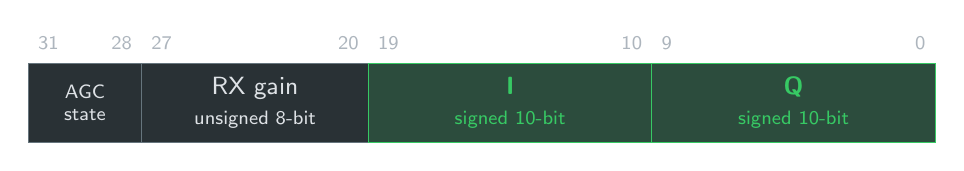
\begin{tikzpicture}[x=.36cm, y=1cm, font=\sffamily\small, text=foreground]
  \draw[fill=surface, draw=outline] (0,0) rectangle (4,1);
  \draw[fill=surface, draw=outline] (4,0) rectangle (12,1);
  \draw[fill=accent!18!surface, draw=accent] (12,0) rectangle (22,1);
  \draw[fill=accent!18!surface, draw=accent] (22,0) rectangle (32,1);
  \node[align=center, font=\scriptsize] at (2,.5) {AGC\\state};
  \node[align=center] at (8,.5) {RX gain\\{\scriptsize unsigned 8-bit}};
  \node[align=center, text=accent] at (17,.5) {\textbf{I}\\{\scriptsize signed 10-bit}};
  \node[align=center, text=accent] at (27,.5) {\textbf{Q}\\{\scriptsize signed 10-bit}};
  \foreach \x/\bit in {0/31,4/27,12/19,22/9} {
    \node[anchor=south west, font=\scriptsize, text=muted] at (\x,1.05) {\bit};
  }
  \foreach \x/\bit in {4/28,12/20,22/10,32/0} {
    \node[anchor=south east, font=\scriptsize, text=muted] at (\x,1.05) {\bit};
  }
\end{tikzpicture}
\end{document}
